\documentclass[aspectratio=169,10pt]{beamer}

% ==============================================================================
% THEME & MODERN CLEAN PALETTE
% ==============================================================================
\usetheme{Madrid}
\usecolortheme{whale}
\usefonttheme{professionalfonts}

% Premium Academic Colors
\definecolor{navyblue}{RGB}{0,32,96}
\definecolor{headerblue}{RGB}{16,48,112}
\definecolor{accentblue}{RGB}{24,76,152}
\definecolor{darkgreen}{RGB}{12,112,48}
\definecolor{crimsonred}{RGB}{165,24,24}
\definecolor{amberorange}{RGB}{210,105,12}
\definecolor{softblue}{RGB}{240,246,255}
\definecolor{softgreen}{RGB}{238,252,242}
\definecolor{softorange}{RGB}{255,248,236}
\definecolor{softred}{RGB}{255,240,240}
\definecolor{softpurple}{RGB}{245,240,255}
\definecolor{cardgray}{RGB}{248,250,252}
\definecolor{borderblue}{RGB}{35,85,160}
\definecolor{bordergreen}{RGB}{25,125,55}
\definecolor{borderorange}{RGB}{195,95,15}
\definecolor{borderred}{RGB}{165,35,35}
\definecolor{borderpurple}{RGB}{115,55,165}

% Beamer Element Styling
\setbeamercolor{palette primary}{bg=navyblue,fg=white}
\setbeamercolor{palette secondary}{bg=accentblue,fg=white}
\setbeamercolor{palette tertiary}{bg=headerblue,fg=white}
\setbeamercolor{frametitle}{bg=headerblue,fg=white}
\setbeamercolor{titlelike}{parent=palette primary}
\setbeamercolor{block title}{bg=accentblue,fg=white}
\setbeamercolor{block body}{bg=softblue,fg=black}
\setbeamercolor{block title example}{bg=darkgreen,fg=white}
\setbeamercolor{block body example}{bg=softgreen,fg=black}
\setbeamercolor{block title alerted}{bg=crimsonred,fg=white}
\setbeamercolor{block body alerted}{bg=softred,fg=black}

% Clean Margins & Templates
\setbeamersize{text margin left=8mm, text margin right=8mm}
\setbeamertemplate{navigation symbols}{}
\setbeamertemplate{headline}{}

% Streamlined Footline
\setbeamertemplate{footline}{
    \leavevmode%
    \hbox{%
    \begin{beamercolorbox}[wd=.45\paperwidth,ht=2.4ex,dp=0.8ex,left]{palette primary}%
        \hspace*{3ex}\textbf{Part 2: Custom Backbone Architecture (RoPE + Sparse Attention)}
    \end{beamercolorbox}%
    \begin{beamercolorbox}[wd=.35\paperwidth,ht=2.4ex,dp=0.8ex,center]{palette secondary}%
        Frequency-Adaptive 2D RoPE \& Spatial-Semantic Attention
    \end{beamercolorbox}%
    \begin{beamercolorbox}[wd=.20\paperwidth,ht=2.4ex,dp=0.8ex,right]{palette primary}%
        Slide \insertframenumber{} / 5\hspace*{3ex}
    \end{beamercolorbox}}%
    \vskip0pt%
}

% ==============================================================================
% PACKAGES
% ==============================================================================
\usepackage[utf8]{inputenc}
\usepackage[T5]{fontenc}
\usepackage[vietnamese]{babel}
\usepackage{amsmath,amssymb,amsfonts,mathtools,bm}
\usepackage{graphicx}
\usepackage{booktabs}
\usepackage{tikz}
\usetikzlibrary{shapes.geometric, arrows.meta, positioning, calc, fit, backgrounds}

\graphicspath{{../output/}{output/}{../}{./}}

% ==============================================================================
% DOCUMENT BEGIN
% ==============================================================================
\begin{document}

% ==============================================================================
% SLIDE 1: MOTIVATION & PROBLEM STATEMENT
% ==============================================================================
\begin{frame}{1. Động Lực Cải Tiến Kiến Trúc (Motivation)}
\vspace{-0.2em}
Trong mô hình DINOv1 gốc (\texttt{ViT-Small/16}), hai thành phần cốt lõi gặp phải hạn chế lớn:

\vspace{0.4em}
\begin{columns}[t]
    % Problem 1: APE Limitation
    \begin{column}{0.48\textwidth}
        \begin{alertblock}{\textbf{Hạn chế 1: Mã hóa Vị trí Tuyệt đối (APE)}}
            \small
            \begin{itemize}\setlength{\itemsep}{6pt}
                \item \textbf{Méo hình học khi Multi-Crop}: DINO huấn luyện đồng thời ảnh $224\times 224$ (196 patch) và $96\times 96$ (36 patch). Bảng APE buộc phải nội suy bicubic $\Rightarrow$ gây sai lệch tương quan khoảng cách.
                \item \textbf{Thiếu tính bất biến tịnh tiến}: Không mô hình hóa trực tiếp khoảng cách tương đối giữa hai patch $(\Delta x, \Delta y)$.
            \end{itemize}
        \end{alertblock}
    \end{column}

    % Problem 2: Full Attention Limitation
    \begin{column}{0.48\textwidth}
        \begin{alertblock}{\textbf{Hạn chế 2: Full Dense Attention $\mathcal{O}(N^2)$}}
            \small
            \begin{itemize}\setlength{\itemsep}{6pt}
                \item \textbf{Lãng phí tính toán nghiêm trọng}: Mọi token đều tương tác với toàn bộ $197$ token, trong khi $>85\%$ trọng số sau hội tụ xấp xỉ bằng $0$.
                \item \textbf{Nhiễu nền (Background Clutter)}: Cơ chế Dense Attention khiến token \texttt{[CLS]} dễ bị phân tán vào nền trời, cỏ và bối cảnh xung quanh thay vì tập trung vào vật thể chính.
            \end{itemize}
        \end{alertblock}
    \end{column}
\end{columns}

\vspace{0.6em}
\begin{exampleblock}{\textbf{Mục tiêu Đề xuất}}
    \centering\small
    Thay thế APE bằng \textbf{Frequency-Adaptive 2D RoPE} \& thay thế Dense Attention bằng \textbf{Spatial-Semantic Sparse Attention}.
\end{exampleblock}
\end{frame}

% ==============================================================================
% SLIDE 2: OVERVIEW OF THE 2 ARCHITECTURAL ENHANCEMENTS
% ==============================================================================
\begin{frame}{2. Tổng Quan Kiến Trúc Đề Xuất (Architecture Overview)}
\vspace{-0.3em}
\begin{columns}[c]
    % Left Column: TikZ Comparison Diagram
    \begin{column}{0.58\textwidth}
        \centering
        \resizebox{\textwidth}{!}{%
        \begin{tikzpicture}[
            font=\sffamily\footnotesize,
            >=Latex,
            box/.style={draw=black!70, rounded corners=3pt, align=center, inner sep=4pt, line width=0.65pt},
            bluebox/.style={box, fill=softblue, draw=borderblue},
            greenbox/.style={box, fill=softgreen, draw=bordergreen},
            orangebox/.style={box, fill=softorange, draw=borderorange},
            redbox/.style={box, fill=softred, draw=borderred},
            graybox/.style={box, fill=cardgray, draw=black!55},
            arrow/.style={->, line width=0.85pt, draw=black!75}
        ]
            % Baseline Block
            \begin{scope}[local bounding box=colBase]
                \node[font=\bfseries\small, text=crimsonred] (tb) at (0, 0) {Baseline DINO ViT Block};
                \node[graybox, text width=3.9cm, below=0.25cm of tb] (b1) {Patch Embedding ($16\times 16$)};
                \node[redbox, text width=3.9cm, below=0.28cm of b1] (b2) {\textbf{+ Learnable APE Table}\\ \scriptsize Bị méo khi nội suy $96\times 96$};
                \node[graybox, text width=3.9cm, below=0.28cm of b2] (b3) {LayerNorm + Q,K,V Projection};
                \node[redbox, text width=3.9cm, below=0.28cm of b3] (b4) {\textbf{Full Dense Attention}\\ \scriptsize $197\times 197$ ma trận đầy đủ};
                \node[graybox, text width=3.9cm, below=0.28cm of b4] (b5) {LayerNorm + MLP ($384\to 1536$)};
                \draw[arrow] (b1) -- (b2);
                \draw[arrow] (b2) -- (b3);
                \draw[arrow] (b3) -- (b4);
                \draw[arrow] (b4) -- (b5);
            \end{scope}

            % Proposed Block
            \begin{scope}[local bounding box=colProp, xshift=5.4cm]
                \node[font=\bfseries\small, text=darkgreen] (tp) at (0, 0) {Proposed ViT Block (Ours)};
                \node[graybox, text width=4.3cm, below=0.25cm of tp] (p1) {Patch Embedding ($16\times 16$)\\ \scriptsize \textcolor{darkgreen}{\textbf{Loại bỏ bảng APE không gian}}};
                \node[graybox, text width=4.3cm, below=0.28cm of p1] (p2) {LayerNorm + Q,K,V Projection};
                \node[orangebox, text width=4.3cm, below=0.28cm of p2] (p3) {\textbf{Component 1: 2D RoPE}\\ \scriptsize Xoay trực tiếp vector $Q, K$\\ \scriptsize Token \texttt{[CLS]} giữ nguyên ($\mathbf{R}=\mathbf{I}$)};
                \node[greenbox, text width=4.3cm, below=0.28cm of p3] (p4) {\textbf{Component 2: Sparse Attention}\\ \scriptsize Cục bộ $3\times 3$ + Top-$16$ + \texttt{[CLS]}\\ \scriptsize \textbf{26 active keys} ($-86.8\%$ tính toán)};
                \node[graybox, text width=4.3cm, below=0.28cm of p4] (p5) {LayerNorm + MLP ($384\to 1536$)};
                \draw[arrow] (p1) -- (p2);
                \draw[arrow] (p2) -- (p3);
                \draw[arrow] (p3) -- (p4);
                \draw[arrow] (p4) -- (p5);
            \end{scope}

            \begin{scope}[on background layer]
                \node[draw=crimsonred!40, dashed, rounded corners=4pt, fit=(colBase), inner sep=5pt] {};
                \node[draw=darkgreen!60, dashed, rounded corners=4pt, fit=(colProp), inner sep=5pt] {};
            \end{scope}
        \end{tikzpicture}%
        }
    \end{column}

    % Right Column: High-Level Highlights
    \begin{column}{0.40\textwidth}
        \begin{block}{\textbf{Nguyên Lý Cốt Lõi}}
            \small
            \begin{itemize}\setlength{\itemsep}{5pt}
                \item \textbf{Giữ nguyên 100\% tham số}:\\
                Backbone đạt đúng \textbf{21,665,664} tham số (bằng tuyệt đối với mô hình gốc).
                \item \textbf{Bảo toàn FLOPs lý thuyết}:\\
                \textbf{9.20 GFLOPs} tại độ phân giải $224\times 224$.
                \item \textbf{Tính toán cục bộ \& toàn cục}:\\
                2D RoPE nhúng tọa độ liên tục; Sparse Attention gom đúng 26 khóa nổi bật ngữ nghĩa.
            \end{itemize}
        \end{block}
    \end{column}
\end{columns}
\end{frame}

% ==============================================================================
% SLIDE 3: COMPONENT 1 — FREQUENCY-ADAPTIVE 2D RoPE
% ==============================================================================
\begin{frame}{3. Component 1: Frequency-Adaptive 2D Rotary Position Embedding}
\vspace{-0.2em}
\begin{columns}[t]
    % Column 1: Formulation & Relative Property
    \begin{column}{0.48\textwidth}
        \begin{block}{\textbf{Cơ Chế Xoay Vector 2D Không Gian}}
            \small
            Phân chia chiều không gian head $d_h = 64$ thành 2 trục $x, y$:
            \vspace{-0.2em}
            \[ d_x = d_y = 32, \quad M = 16 \text{ dải tần số } \omega_m \]
            Vector $Q$ và $K$ được xoay qua ma trận trực giao $\mathbf{R}_{\Theta}$:
            \vspace{-0.2em}
            \[ \tilde{\mathbf{q}}_i = \mathbf{R}_{\Theta}(p_{x,i}, p_{y,i}) \mathbf{q}_i, \quad \tilde{\mathbf{k}}_j = \mathbf{R}_{\Theta}(p_{x,j}, p_{y,j}) \mathbf{k}_j \]
            \textbf{Bất biến tịnh tiến tương đối qua tích vô hướng}:
            \vspace{-0.2em}
            \[ \langle \tilde{\mathbf{q}}_i, \tilde{\mathbf{k}}_j \rangle = \mathbf{q}_i^T \mathbf{R}_{\Theta}(p_{x,i}-p_{x,j}, \, p_{y,i}-p_{y,j}) \mathbf{k}_j \]
            $\Rightarrow$ Tự động mã hóa khoảng cách hình học tương đối!
        \end{block}
    \end{column}

    % Column 2: Coordinate Blending & CLS
    \begin{column}{0.48\textwidth}
        \begin{exampleblock}{\textbf{Lịch Phối Trộn Tọa Độ Thích Ứng Tần Số}}
            \small
            Trộn tọa độ nguyên tuyệt đối và chuẩn hóa:
            \vspace{-0.2em}
            \[ p_m = \alpha_m \cdot p_{\text{raw}} + (1 - \alpha_m) \cdot p_{\text{norm}}, \quad \alpha_m = 1 - \frac{m}{M-1} \]
            \begin{itemize}\setlength{\itemsep}{3pt}
                \item \textbf{Tần số cao ($\alpha \to 1$)}: Tọa độ nguyên $\Rightarrow$ nắm bắt chi tiết texture và ranh giới sắc nét.
                \item \textbf{Tần số thấp ($\alpha \to 0$)}: Tọa độ chuẩn hóa $\Rightarrow$ bất biến tỷ lệ xuyên qua các crop $224^2$ và $96^2$.
            \end{itemize}
        \end{exampleblock}

        \vspace{0.2em}
        \begin{alertblock}{\textbf{Bảo Toàn Token \texttt{[CLS]}}}
            \small
            \texttt{[CLS]} không có tọa độ không gian: gán $\boldsymbol{\theta}_{\text{cls}} = \mathbf{0} \Rightarrow \mathbf{R} = \mathbf{I}$.\\
            $\Rightarrow$ Tránh gây thiên kiến không gian giả tạo cho nhãn toàn cục.
        \end{alertblock}
    \end{column}
\end{columns}
\end{frame}

% ==============================================================================
% SLIDE 4: COMPONENT 2 — SPATIAL-SEMANTIC SPARSE ATTENTION
% ==============================================================================
\begin{frame}{4. Component 2: Spatial-Semantic Sparse Softmax Attention}
\vspace{-0.3em}
\begin{columns}[c]
    % Column 1: TikZ Visual Grid Support
    \begin{column}{0.48\textwidth}
        \centering
        \resizebox{0.92\textwidth}{!}{%
        \begin{tikzpicture}[
            font=\sffamily\footnotesize,
            box/.style={draw=black!70, rounded corners=3pt, align=center, inner sep=4pt}
        ]
            % CLS Token node
            \node[box, fill=softpurple, draw=borderpurple, text width=5.2cm] (cls) {
                \textbf{Cầu Nối Hai Chiều \texttt{[CLS]} (Index 0)}\\
                \scriptsize \texttt{[CLS]} nhìn mọi token \& mọi token đều nhìn \texttt{[CLS]}
            };

            % 5x5 Grid
            \coordinate (gtop) at ([yshift=-0.35cm]cls.south);
            \def\cs{0.50}
            \begin{scope}[shift={($(gtop)+(-2.5*\cs, -5*\cs)$)}]
                \foreach \r in {0,...,4} {
                    \foreach \c in {0,...,4} {
                        \filldraw[fill=white, draw=black!35, line width=0.4pt]
                            (\c*\cs, \r*\cs) rectangle ++(\cs, \cs);
                    }
                }
                % 3x3 Local window
                \foreach \r in {1,2,3} {
                    \foreach \c in {1,2,3} {
                        \filldraw[fill=softgreen, draw=bordergreen, line width=0.55pt]
                            (\c*\cs, \r*\cs) rectangle ++(\cs, \cs);
                    }
                }
                % Query center
                \filldraw[fill=navyblue, draw=black, line width=0.7pt]
                    (2*\cs, 2*\cs) rectangle ++(\cs, \cs)
                    node[pos=0.5, text=white, font=\bfseries\small] {$q_i$};
                % Semantic Top-K
                \filldraw[fill=softorange, draw=borderorange, line width=0.55pt]
                    (0*\cs, 4*\cs) rectangle ++(\cs, \cs) node[pos=0.5, font=\scriptsize\bfseries] {Top-$K$};
                \filldraw[fill=softorange, draw=borderorange, line width=0.55pt]
                    (4*\cs, 4*\cs) rectangle ++(\cs, \cs) node[pos=0.5, font=\scriptsize\bfseries] {Top-$K$};
                \filldraw[fill=softorange, draw=borderorange, line width=0.55pt]
                    (4*\cs, 0*\cs) rectangle ++(\cs, \cs) node[pos=0.5, font=\scriptsize\bfseries] {Top-$K$};
                \filldraw[fill=softorange, draw=borderorange, line width=0.55pt]
                    (0*\cs, 1*\cs) rectangle ++(\cs, \cs) node[pos=0.5, font=\scriptsize\bfseries] {Top-$K$};
            \end{scope}

            \draw[<->, line width=1.0pt, draw=borderpurple] (cls.south) -- ++(0, -0.28);
        \end{tikzpicture}%
        }
    \end{column}

    % Column 2: 3 Pathways & Exact Softmax
    \begin{column}{0.50\textwidth}
        \begin{block}{\textbf{3 Nhánh Hỗ Trợ Hoạt Động $\mathcal{S}_i$}}
            \small
            Tập khóa hoạt động: $\mathcal{S}_i = \mathcal{N}_{\text{local}}(i) \cup \mathcal{N}_{\text{semantic}}(i) \cup \{0\}$
            \begin{enumerate}\setlength{\itemsep}{3pt}
                \item \textcolor{bordergreen}{\textbf{Cục bộ $3\times 3$ ($\mathcal{N}_{\text{local}}$)}}: 9 patch lân cận (Chebyshev $R=1$).
                \item \textcolor{borderorange}{\textbf{Ngữ nghĩa Top-$K$ ($\mathcal{N}_{\text{semantic}}$)}}: 16 patch có độ tương đồng tích vô hướng cao nhất.
                \item \textcolor{borderpurple}{\textbf{Cầu nối \texttt{[CLS]}}}: Index $0$ kết nối ngữ cảnh toàn cục.
            \end{enumerate}
            $\Rightarrow$ \textbf{Tổng khóa kích hoạt: 26 / 197 keys (Giảm 86.8\% phép tính)}.
        \end{block}

        \vspace{0.2em}
        \begin{exampleblock}{\textbf{Chuẩn Hóa Softmax Chính Xác}}
            \small
            \vspace{-0.2em}
            \[ \mathbf{A}_{ij} = \frac{\exp(\tilde{\mathbf{q}}_i^T \tilde{\mathbf{k}}_j / \sqrt{d_h})}{\sum_{l \in \mathcal{S}_i} \exp(\tilde{\mathbf{q}}_i^T \tilde{\mathbf{k}}_l / \sqrt{d_h})} \quad \forall j \in \mathcal{S}_i \]
            \textbf{Không xấp xỉ}: Trọng số tổng đúng bằng 1, triệt tiêu gradient vanishing và tránh hiện tượng tràn số.
        \end{exampleblock}
    \end{column}
\end{columns}
\end{frame}

% ==============================================================================
% SLIDE 5: VISUAL VERIFICATION & PERFORMANCE GAINS
% ==============================================================================
\begin{frame}{5. Minh Chứng Trực Quan: Attention Maps \& Hiệu Năng}
\vspace{-0.3em}
\begin{columns}[c]
    % Left Column: Real Attention Map Sample
    \begin{column}{0.54\textwidth}
        \begin{block}{\textbf{So Sánh Attention Map 6 Heads (Epoch 190)}}
            \centering
            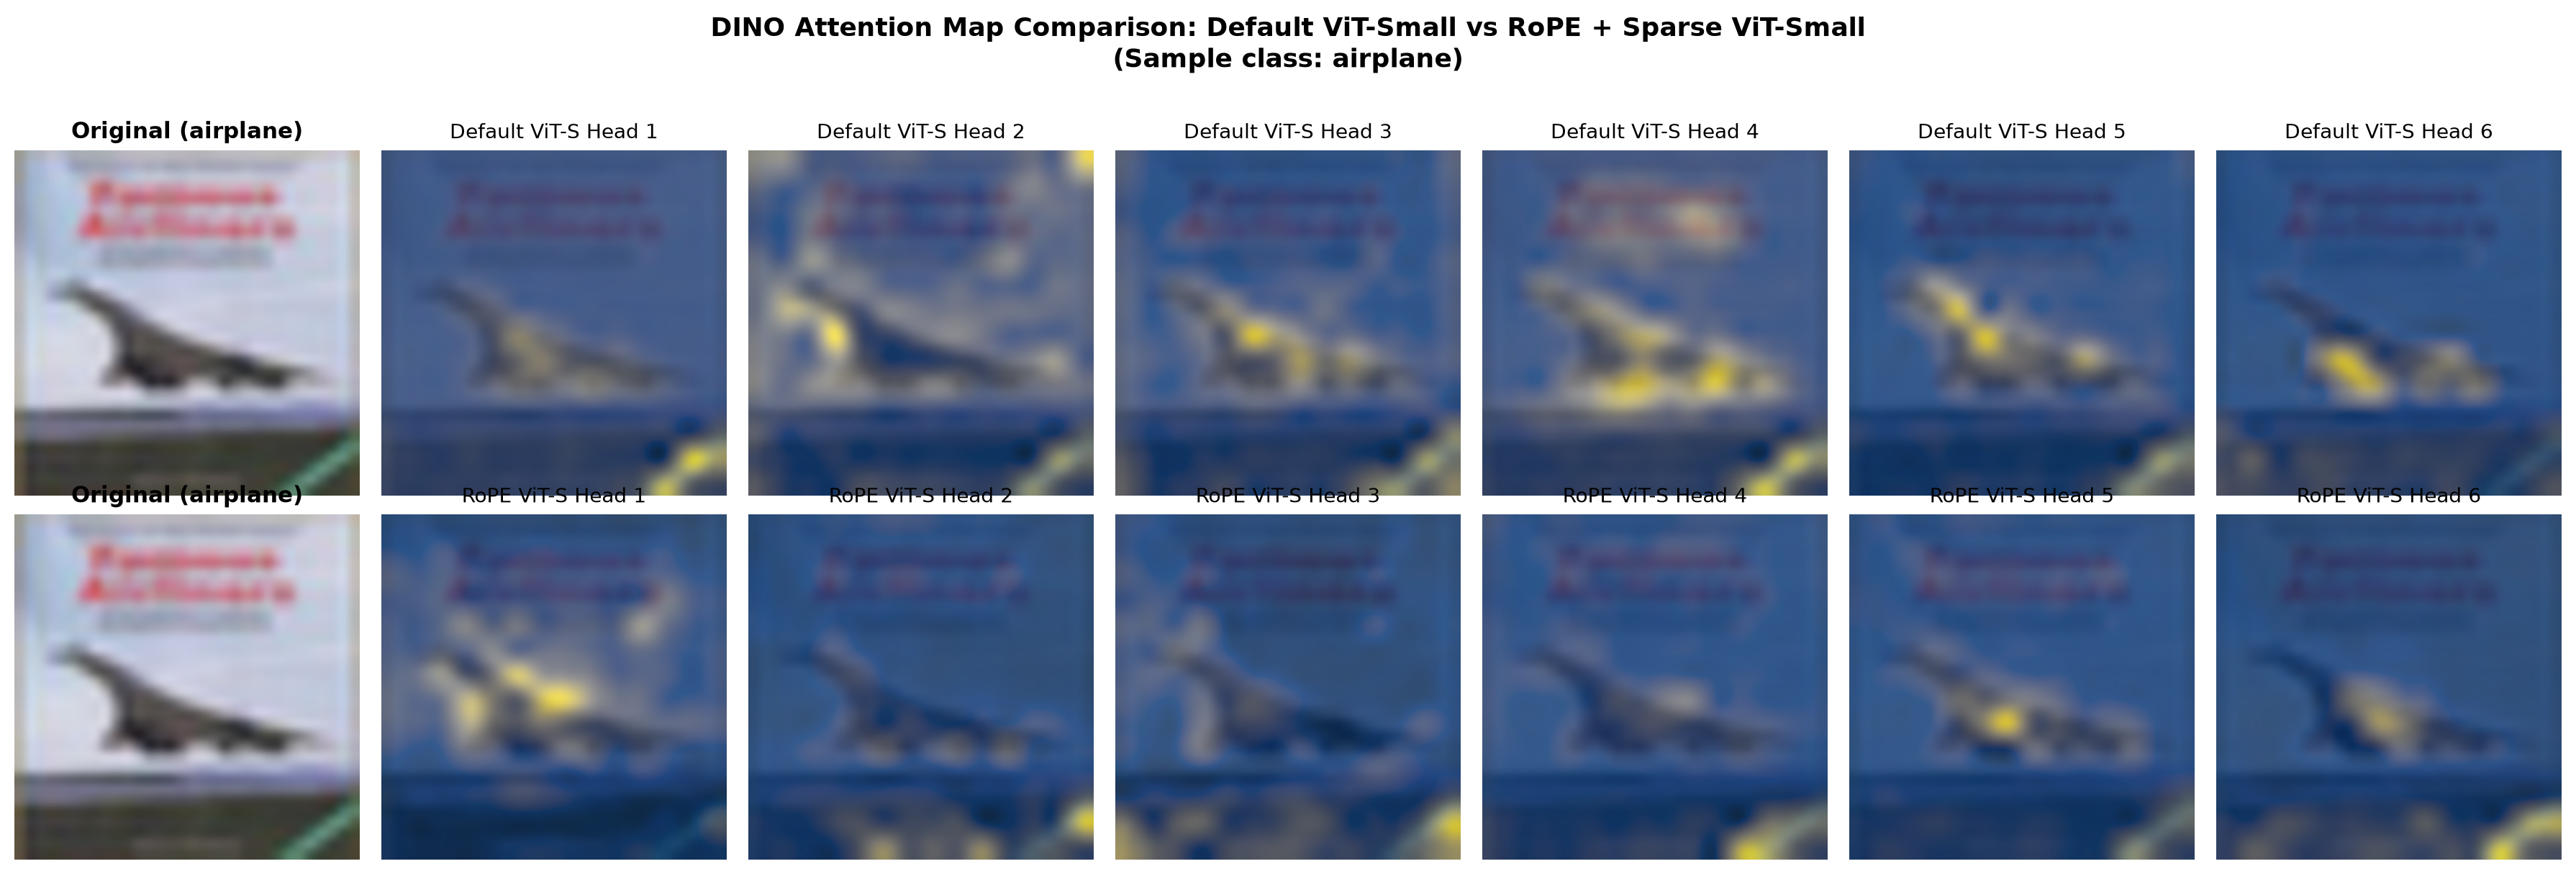
\includegraphics[width=\textwidth]{output/attention_comparison.png}
        \end{block}
        \vspace{-0.2em}
        \begin{exampleblock}{\textbf{Phân Tích Định Tính}}
            \scriptsize
            \begin{itemize}\setlength{\itemsep}{2pt}
                \item \textbf{Baseline ViT}: Chú ý bị phân tán rộng vào nền trời phía sau.
                \item \textbf{RoPE + Sparse (Ours)}: Head 2 và Head 5 gom chặt sự chú ý vào đúng khung thân, cánh và đuôi máy bay, tách bạch hoàn toàn khỏi nền.
            \end{itemize}
        \end{exampleblock}
    \end{column}

    % Right Column: Quantitative Gains & Conclusion
    \begin{column}{0.44\textwidth}
        \begin{exampleblock}{\textbf{Cải Thiện Định Lượng (CIFAR-10)}}
            \small
            \begin{itemize}\setlength{\itemsep}{4pt}
                \item \textbf{k-NN Top-1 ($k=10$)}:\\
                $74.41\% \to \mathbf{75.97\%}$ (\textcolor{darkgreen}{\textbf{+1.56\% gain}}).
                \item \textbf{Linear Probing Top-1}:\\
                $81.46\% \to \mathbf{83.98\%}$ (\textcolor{darkgreen}{\textbf{+2.52\% gain}}).
                \item \textbf{Tốc độ hội tụ phân loại}:\\
                Epoch 10: $73.76\% \to \mathbf{79.86\%}$ (\textcolor{darkgreen}{\textbf{+6.10\%}}).
            \end{itemize}
        \end{exampleblock}
        \vspace{-0.2em}
        \begin{block}{\textbf{Kết Luận Phần 2}}
            \footnotesize
            2D RoPE + Sparse Attention giải quyết trọn vẹn bài toán bảo toàn hình học và khử nhiễu nền mà \textbf{không tăng chi phí tham số}.
        \end{block}
    \end{column}
\end{columns}
\end{frame}

\end{document}
